\documentclass[12pt,a4paper,titlepage,final]{article}

% velikost stranky
\usepackage[top=2.5cm, left=2cm, text={17cm, 25cm}, ignorefoot]{geometry}

%%% ENCODING AND LANGUAGE
\usepackage[czech]{babel}
\usepackage[utf8]{inputenc}

%%% Hyperlinks
\usepackage[bookmarksopen,colorlinks,plainpages=false,urlcolor=blue,unicode,linkcolor=blue]{hyperref}
\usepackage{url}

%%% Tables
\usepackage{multirow}
\usepackage{booktabs}

%%% Figures
\usepackage{graphicx}

%%% Math
\usepackage{mathtools}
\usepackage{amsfonts}

%%% Vlastni prikazy
\newcommand{\matr}[1]{\mathbf{#1}}

%%%%%%%%%%%%%%%%%%%%%%%%%%%%%%%%%%%%%%%%%%%%%%%%%%
%%%%%%%%%%%%%%%%%%%%%%%%%%%%%%%%%%%%%%%%%%%%%%%%%%
%%%%%%%%%%%%%%%%%%%%%%%%%%%%%%%%%%%%%%%%%%%%%%%%%%
\begin{document}


\pagenumbering{arabic}
\setcounter{page}{1}

%%%%%%%%%%%%%%%%%%%%%%%%%%%%%%%%%%%%%%%%%%%%%%%%%%
%%%%%%%%%%%%%%%%%%%%%%%%%%%%%%%%%%%%%%%%%%%%%%%%%%
% title
    
\begin{centering}
\textsc{\textbf{PRL Paralelní a distribuované algoritmy} \\
FIT VUT Brno\\
}

\rule{\textwidth}{1.6pt}\vspace*{-\baselineskip}\vspace*{25pt} 

\begin{LARGE}
\textsc{Mesh Multiplication}
\end{LARGE}

\rule{\textwidth}{1.6pt}\\ % Thick horizontal line

\vspace*{5pt} 
\begin{footnotesize}
\today
\end{footnotesize}
\vspace*{5pt} 

\begin{large}
Jan Bednařík (xbedna45)\\
\end{large}

\end{centering}

%%%%%%%%%%%%%%%%%%%%%%%%%%%%%%%%%%%%%%%%%%%%%%%%%%
%%%%%%%%%%%%%%%%%%%%%%%%%%%%%%%%%%%%%%%%%%%%%%%%%%
% Obsah

%%%%%%%%%%%%%%%%%%%%%%%%%%%%%%%%%%%%%%%%%%%%%%%%%%
\section{Úvod}
V tomto dokumentu je popsána problematika maticového násobení pomocí algoritmu \texttt{Mesh multiplication} na multiprocesorovém systému. Práce vznikla v rámci projektu v kurzu Paralelní a distribuované algoritmy (PRL), kdy bylo úkolem algoritmus implementovat v jazyce \texttt{C++} s použitím knihovny \texttt{OpenMPI} a experimentálně ověřit jeho předpokládanou časovou složitost.

%%%%%%%%%%%%%%%%%%%%%%%%%%%%%%%%%%%%%%%%%%%%%%%%%%
\section{Rozbor algoritmu}
Algoritmus staví na topologii 2rozměrná mřížka procesorů, jež svými rozměry odpovídá rozměrům matice výsledku maticového násobení. Nechť $\matr{A}$, $\matr{B}$, $\matr{C}$ jsou matice, platí $\matr{C} = \matr{A}\matr{B}$, rozměry matice $\matr{A}$ jsou $m \times n$ a rozměry matice $\matr{B}$ jsou $n \times k$. Následující odstavce podávají odvození časové a paměťové složitosti a potřebný počet procesorů.

\paragraph{Časová složitost}
Řádky matice $\matr{A}$ a sloupce matice $\matr{B}$ jsou postupně čteny procesory v prvním sloupci a v prvním řádku 2rozměrné mřížky, přičemž každý procesor následně prvky zasílá procesoru napravo a procesoru dole. Každý řádek $i_{a}$ matice $\matr{A}$ je při horizontálním průchodu mřížkou o jeden krok opožděn oproti řádku $i_{a} - 1$ a stejně tak každý sloupec $j_{b}$ matice $\matr{B}$ je při vertikálním průchodu mřížkou procesorů o jeden krok opožděn oproti sloupci $j_{b} - 1$, díky čemuž se v každém kroku algoritmu do každého procesoru $P_{i_{c}j_{c}}$ dostanou odpovídající si hodnoty matic $\matr{A}$ a $\matr{B}$. Časová složitost potom odpovídá počtu kroků $s$ potřebných k tomu, aby byl poslední řádek matice $\matr{A}$ a poslední sloupec matice $\matr{B}$ zpracován procesorem $P_{mk}$:

\begin{equation}
s = (m - 1) + (k - 1) + n = m + n + k -2
\end{equation}

Časová složitost algoritmu je tedy \textit{lineární}, $O(N)$.

\paragraph{Počet procesorů}
Procesory tvoří 2rozměrnou mřížku odpovídající rozměrům výsledné matice. Počet procesorů lze tedy vyjádřit jako $P = m * k$, jedná se o \textit{kvadratickou} složitost $O(N^{2})$.

\paragraph{Paměťová složitost}
Každý procesor disponuje pouze pamětí pro dvě vstupní hodnoty a akumulátorem, paměťová složitost je tak \textit{lineární}, $O(N)$

\paragraph{Cena}
Cena algoritmu je dána jako násobek počtu procesorů a časové složitosti, tedy $C(N) = N^{2}*N = N^{3}$. Algoritmus \texttt{Mesh multiplication} není optimální.

%%%%%%%%%%%%%%%%%%%%%%%%%%%%%%%%%%%%%%%%%%%%%%%%%%
\section{Implementace}
Program je implementován v \texttt{C++} s použitím knihovny \texttt{OpenMPI}, jež staví na zasílání zpráv mezi procesory. Komunikační protokol použitý pro implementaci algoritmu \textit{Mesh multiplication} je znázorněný ve schématu \ref{fig:SequenceDiagram}. 

\begin{figure}[!hbt]
	\centering
	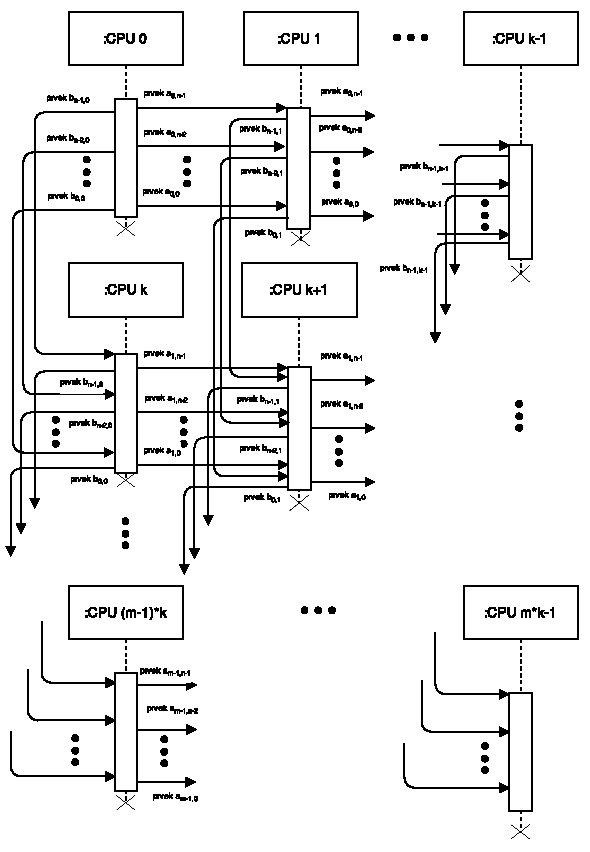
\includegraphics[width=0.75\linewidth]{img/sequence_diagram.pdf}
	\caption{Komunikační protokol procesorů vyjádřený sekvenčním diagramem pro vstupní matice $\matr{A}$ a $\matr{B}$ obecných rozměrů $m \times n$ a $n \times k$.}
	\label{fig:SequenceDiagram}
\end{figure}

Oproti teoretickému popisu průběhu algoritmu se implementace liší tím, že veškerá vstupní data načítá pouze procesor $P_{00}$ a stará se o zasílání hodnot všem procesorům v prvním řádku a prvním sloupci 2rozměrné mřížky procesorů.

%%%%%%%%%%%%%%%%%%%%%%%%%%%%%%%%%%%%%%%%%%%%%%%%%%
\section{Experimenty}
Běh algoritmu byl otestován na jednoprocesorovém systému (2 jádra, 4 vlákna) ve virtualizovaném prostředí operačního systému \texttt{Lubuntu 14.04}. Testovány byly vstupní čtvercové matice o stejných rozměrech $n \times n$, kde $n \in \mathbb{N}, 1 \leq n \leq 13$. Čas běhu staví na knihovní funkci \texttt{MPI::Wtime()} pro přesné měření času. Měření provádí pouze první procesor, kdy spouští časovač po načtení všech vstupních dat a před započetím zasílání prvků ostatním procesorům. Jakmile přijme výslednou hodnotu od posledního procesoru ($P_{mk}$), zastaví časovač. Doba běhu tak není zatížena vstupně výstupními operacemi.

Výsledky měření jsou uvedeny v grafu \ref{fig:CasVSPocetPrvku}. Měřené časy pro jednotlivé velikosti vstupních matic jsou proloženy přímkou znázorňující očekávaný lineární průběh. Jak je z grafu patrné, lineární průběh je respektován pouze při nižších velikostech matic, zatímco se zvyšující se velikostí matic časovou složitost lépe modeluje kubický průběh. Tento je způsoben faktem, že byl systém testován na jednoprocesorovém systému, kde jsou fyzické procesory emulovány jako procesy, tedy vlivem nutnosti přepínat kontext paralelní zpracování postupně degraduje na sekvenční.

\begin{figure}[!hbt]
	\centering
	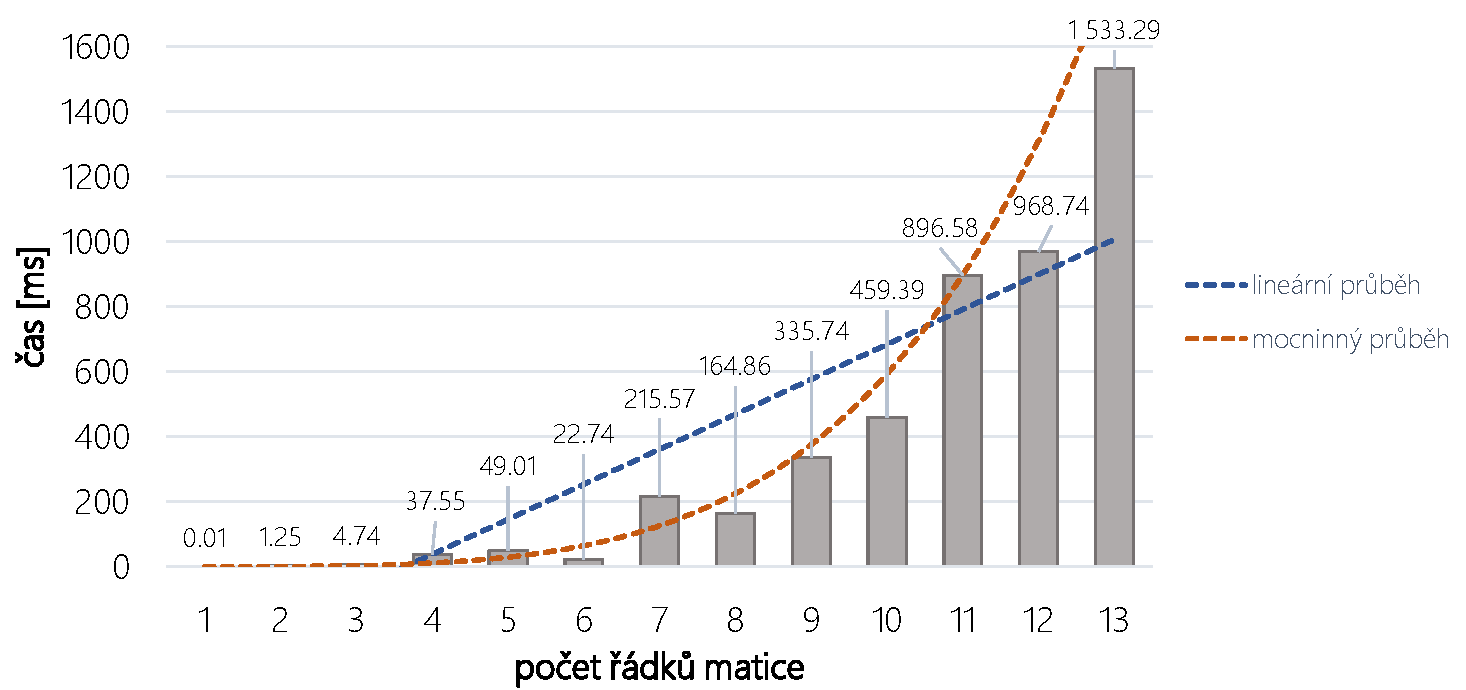
\includegraphics[width=1.0\linewidth]{img/graf.pdf}
	\caption{Závislost doby běhu programu na počtu vstupních prvků.}
	\label{fig:CasVSPocetPrvku}
\end{figure}

Pro dosažení co nejvěrnějších výsledků byl pro každou délku posloupnosti $N$ test proveden desetkrát, z výsledků byly odstraněny dvě nejnižší a tři nejvyšší hodnoty a zbylých pět hodnot bylo průměrováno.

%%%%%%%%%%%%%%%%%%%%%%%%%%%%%%%%%%%%%%%%%%%%%%%%%%
\section{Závěr}
V rámci projektu byl implementován algoritmus \textit{Mesh multiplication}, byla odvozena jeho teoretická časová a paměťová složitost i cena a provedeny experimenty nad reálnými daty. Testy potvrdily lineární časovou složitost algoritmu, přesto byly zaznamenány nezanedbatelné odchylky. Ty jsou způsobené především proto, že je testovací stroj jednoprocesorový, tedy jednotlivé procesory požadované algoritmem jsou nahrazeny procesy sdílejícími výpočetní prostředky a neběží tak zcela paralelně. Při vyšších rozměrech vstupních matic tak složitost postupně degraduje na mocninnou podobně jako u sekvenčního přístupu.

%%%%%%%%%%%%%%%%%%%%%%%%%%%%%%%%%%%%%%%%%%%%%%%%%%


\end{document}
